\documentclass{standalone}

\ifstandalone
	\usepackage{amsmath}
	\usepackage{pgfplots}
\fi


\begin{document}
	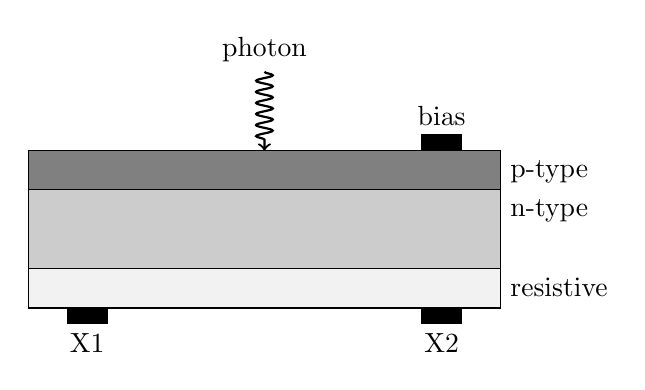
\begin{tikzpicture}
		\filldraw[fill=gray] (0, 1.5) rectangle +(6, 0.5) node[below right]{p-type};
		\filldraw[fill=gray!40] (0, 0.5) rectangle +(6, 1) node[below right]{n-type};
		\filldraw[fill=gray!10] (0, 0) rectangle +(6, 0.5) node[below right]{resistive};
		\filldraw[fill=black] (5, 2) rectangle ++(0.5, 0.2) +(-0.25, 0) node[above]{bias};
		\draw [->, thick, decorate, decoration={snake, amplitude=3, segment length=4, post length=3}] (3, 3) node[above]{photon} -- +(0, -1);
		\filldraw[fill=black] (0.5, 0) rectangle ++(0.5, -0.2) +(-0.25, 0) node[below]{X1};
		\filldraw[fill=black] (5, 0) rectangle ++(0.5, -0.2) +(-0.25, 0) node[below]{X2};
	\end{tikzpicture}
\end{document}
